\chapter{Writing: The Reusable Hour}

There are many reasons to learn to write. Some are cultural, some are professional, and some are almost moral. Reading can make a person fuller; discussion can make a person sharper; writing can make a person more complete.

But on the road to wealth freedom, one reason is unusually practical:

\begin{quote}
Writing is one of the few ordinary ways to sell the same stretch of time again and again.
\end{quote}

This is not a metaphor. If you spend an afternoon explaining an idea privately to one person, that afternoon has been sold once. If you spend the same afternoon shaping the idea into an essay that can be read by ten thousand people over many years, the time has been multiplied. If you spend months writing a useful book that continues selling for a decade, those months may be resold hundreds of thousands or millions of times.

The previous chapters have examined normal time trading: raising the price of one unit of time, working for oneself while employed, and learning to buy other people's time responsibly. Writing introduces another route. It does not merely raise the price of one hour. It makes one hour reusable.

This is why writing belongs in a book about wealth freedom. It is not only an artistic activity. It is a personal business model.

\section*{Public Communication}

Private conversation is valuable, but it does not scale well. One person speaks, one person listens, and both must be present at the same time. The exchange may be deep, but the reach is narrow.

Public communication changes the equation.

Speaking to a room, teaching a class, publishing an essay, recording a course, or writing a book all do something similar: they allow one act of communication to serve many people. The time cost does not rise in proportion to the number of listeners or readers.

\begin{center}
\begin{adjustbox}{max width=\linewidth}
\begin{tabular}{lll}
\hline
Mode & Time sold & Limitation \\
\hline
Private advice & Once & One listener at a time \\
Lecture or class & Many times at once & Place and schedule \\
Published writing & Many times over time & Quality and usefulness \\
\hline
\end{tabular}
\end{adjustbox}
\end{center}

The internet made this even more important. A person no longer needs a classroom, a publisher's front table, or a conference hall before his words can travel. Writing can be published immediately and distributed without geographic permission.

This does not mean everyone who writes will be heard. Most writing is ignored, and much of it deserves to be ignored. But the possibility has changed. For an ordinary person, writing is now one of the lowest-cost entrances into scalable communication.

In an age where information moves quickly, communication ability is not decorative. It is a survival skill. The quality of a person's communication affects the quality of resources he can attract: people, opportunities, feedback, trust, capital, and cooperation.

\section*{The Reusable-Time Model}

A job usually pays for time in a straight line. Work one hour, receive one hour's pay. Stop working, stop receiving. This is the basic trap of selling time.

Writing can have a different shape. The time investment is heavy at the beginning. The work must be thought through, written, revised, tested against readers, and improved. But once the work exists, the additional time required for each new reader can approach zero.

\begin{center}
\begin{adjustbox}{max width=\linewidth}
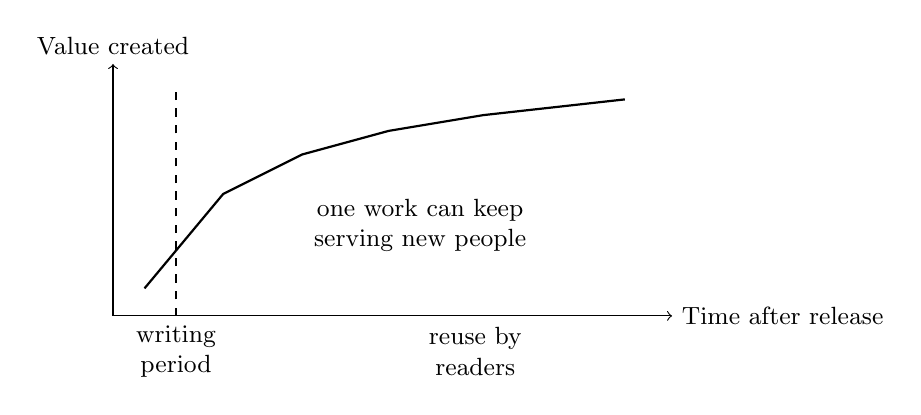
\begin{tikzpicture}[x=1cm,y=1cm,every node/.style={font=\small}]
\draw[->] (0,0) -- (7.1,0) node[right] {Time after release};
\draw[->] (0,0) -- (0,3.2) node[above] {Value created};
\draw[thick] (0.4,0.35) -- (1.4,1.55) -- (2.4,2.05) -- (3.5,2.35) -- (4.7,2.55) -- (6.5,2.75);
\draw[dashed] (0.8,0) -- (0.8,2.9);
\node[align=center] at (0.8,-0.45) {writing\\period};
\node[align=center] at (4.6,-0.45) {reuse by\\readers};
\node[align=center] at (3.9,1.15) {one work can keep\\serving new people};
\end{tikzpicture}
\end{adjustbox}
\end{center}

This model is not guaranteed. A bad book does not become valuable merely because it is printed. A useless essay does not deserve attention merely because it is published. The model works only when the writing remains useful to other people.

But when it does work, the structure is powerful. A useful text can preserve a person's thinking, travel farther than the person can travel, teach while the author sleeps, and keep producing reputation, trust, income, or opportunity long after the original writing time has passed.

This is why a book can be a rare form of ordinary ``one-time labor'' with long aftereffects. It is not literally effortless. Nothing important is. But compared with selling the same hour again tomorrow, and again next week, and again next year, a durable piece of writing has a far better time structure.

\section*{Writing Records Growth}

There is another reason writing is worth doing even before it earns anything:

\begin{quote}
Writing makes growth visible.
\end{quote}

You may remember what you thought about yesterday. But what did you think about last week? Last month? Last year? What question were you struggling with? Which concept did you misunderstand? Which conclusion seemed obvious then but now looks shallow?

Without records, most thinking evaporates.

Writing fixes thought in place. It allows you to return later and see not only what you thought, but how you thought. You can inspect the path. You can see where you were careless, where you were precise, where you borrowed a conclusion, and where you really understood something.

This matters because growth is often too slow to feel from inside the day. A person who writes continuously leaves behind a trail. The trail becomes evidence. It shows whether he has been circling the same vague complaints or actually making progress.

Writing is therefore not merely expression. It is self-measurement.

\section*{The Best Way to Learn}

One of the most effective ways to learn a concept is to teach it to someone else.

Teaching forces clarity. A concept that feels clear while reading often becomes slippery when explained. The gaps appear. The borrowed sentences disappear. The vague parts refuse to cooperate.

Writing is a practical way to teach without first asking for another person's time. You can explain the idea alone. You can revise until the explanation becomes clearer. You can discover which parts you do not understand. Then, after publishing, you can receive feedback from the real world.

This is why writing is a learning machine.

\begin{center}
\begin{adjustbox}{max width=\linewidth}
\begin{tikzpicture}[node distance=1.2cm, every node/.style={font=\small}]
\node[draw, rounded corners, align=center, minimum width=2.5cm, minimum height=0.8cm] (read) {Read};
\node[draw, rounded corners, align=center, minimum width=2.5cm, minimum height=0.8cm, right=of read] (write) {Explain};
\node[draw, rounded corners, align=center, minimum width=2.5cm, minimum height=0.8cm, right=of write] (gap) {Find gaps};
\node[draw, rounded corners, align=center, minimum width=2.5cm, minimum height=0.8cm, below=of write] (revise) {Revise};
\draw[->] (read) -- (write);
\draw[->] (write) -- (gap);
\draw[->] (gap) -- (revise);
\draw[->] (revise) -- (write);
\end{tikzpicture}
\end{adjustbox}
\end{center}

Many people believe they understand because the author's explanation was clear. Then they try to restate the idea in their own words and discover confusion. This discovery is not failure. It is the beginning of real learning.

Taking notes has a similar effect. Research and classroom experience both point in the same direction: the act of recording helps understanding even if the notes are not reread later. The hand, eye, and mind cooperate. The learner becomes active instead of merely exposed.

Good students often use more than one channel. They look, say, write, calculate, redraw, and explain. Writing gathers these channels into one deliberate practice.

\section*{Do Not Wait Until Ready}

A familiar sentence blocks many lives:

\begin{quote}
When I am ready, I will begin.
\end{quote}

It sounds responsible. Often it is only procrastination dressed as responsibility.

Writing is not something you prepare for forever and then begin perfectly. Each piece of writing is preparation for the next piece. The clumsy paragraph prepares the clearer paragraph. The awkward essay prepares the useful essay. The failed explanation prepares the explanation that finally works.

Perfectionism is especially dangerous here because writing exposes thought. When you publish, other people can see your limits. They can see that your examples are weak, your structure is loose, your vocabulary is ordinary, and your thinking is not yet deep enough.

So what?

Everyone begins with ordinary ability. The problem is not being ordinary at the starting line. The problem is insisting on ordinary thinking while claiming extraordinary wishes.

A person who wants wealth freedom must learn to think from the future. The comparison is not between your current self and a successful person's current self. That comparison only produces shame or fantasy. The useful comparison is between your future self, after years of deliberate growth, and the person who is already ahead today.

From that future position, beginning badly is not humiliating. It is necessary.

\section*{Thinking Is Not Enough}

Ideas without execution are usually illusions.

This is harsh, but useful. A person may have brilliant intentions, impressive opinions, and elegant plans. If none of them becomes action, they remain private weather. They do not change reality.

Writing is a simple test. If you say you understand a concept, write it. If you say the idea matters, explain why. If you say it can help others, make it usable. If you cannot do that yet, you have found the work.

This also explains why short public comments can be a reasonable starting point. A comment below an article is not a masterpiece, but it is practice. It forces a small conclusion into words. It places your thinking beside other people's thinking. It gives you comparison, friction, and feedback.

A group of readers who write in response to the same idea can accidentally become a writing school. Each person sees not only the original essay, but many attempts to digest it. Some comments are vague. Some are sharp. Some repeat. Some extend. The comparison teaches.

Do not despise small beginnings. Despise only the refusal to begin.

\section*{The Ultimate Writing Technique}

Many writing tips are useful. Structure matters. Style matters. Titles matter. Stories matter. Rhythm matters. Editing matters.

But one question stands above them:

\begin{quote}
Is this useful to other people?
\end{quote}

This question filters most writing immediately. It also prevents vanity. The goal is not to display that you have read something, felt something, or suffered something. The goal is to create value for the reader.

Once this question is taken seriously, it naturally becomes more precise:

\begin{enumerate}
\item Who is this useful to?
\item How useful is it?
\item How can it become more useful?
\item How many people could use it?
\item For how long will it remain useful?
\item What must be removed because it serves only my ego?
\item If it creates real value, what is an appropriate way for readers to repay that value?
\end{enumerate}

This is the commercial and moral center of writing. If the work helps people, the world has a reason to respond. The response may be money, trust, reputation, opportunities, relationships, invitations, or simply better feedback. But the response begins with usefulness.

Polished uselessness is still useless. Plain usefulness can travel far.

\section*{Writing Trains the Core Abilities}

Not everyone will become wealthy by writing books. Not every successful person is a writer or speaker. Wealth freedom has more than one road.

Still, writing remains worth learning because it trains abilities required on almost every road:

\begin{itemize}
\item learning ability;
\item thinking ability;
\item analytical ability;
\item communication ability.
\end{itemize}

To write well, you must observe. To observe well, you must pay attention. To explain well, you must organize. To organize well, you must analyze. To improve, you must accept feedback. To continue, you must build discipline.

A person who writes regularly begins to treat life differently. Books, films, conversations, work problems, investment decisions, and personal failures all become material for thought. He notices details that used to pass by. He asks what can be learned, what can be explained, and what can be made useful to someone else.

This is why writing is one of the cheapest serious training systems available. The tools are simple. The cost is low. The feedback can be real. The benefits spread into every other domain.

If you can think, analyze, and learn, but cannot communicate, you may lose to people who understand less but communicate better. That is not fair, but it is common. The road to freedom is not improved by complaining about this fact. It is improved by acquiring the missing skill.

\section*{The Practice}

The practice is simple, but not easy.

Write something useful. Publish it somewhere appropriate. Watch the feedback. Rewrite your understanding. Repeat.

Do not begin by asking whether you are talented. Talent is a lazy question. Begin by asking whether the next piece can help someone. Begin by asking whether your explanation is clearer than last week's. Begin by asking whether you can preserve one real thought before it disappears.

A practical writing routine can be modest:

\begin{enumerate}
\item Choose one concept, problem, or observation.
\item Explain it in plain language.
\item Add one concrete example.
\item State who it helps and how.
\item Remove anything that does not serve the reader.
\item Publish or share it where feedback is possible.
\item Keep the draft so future growth has a record.
\end{enumerate}

The point is not to become impressive immediately. The point is to create a loop in which thinking becomes visible, visible thinking can be improved, and improved thinking can serve others.

This loop compounds.

\section*{A Different Kind of Time Sale}

The road to wealth freedom begins with a painful fact: most people survive by selling time. The goal is not to hate this fact, but to transcend it intelligently.

Writing helps in two ways.

First, it can turn one stretch of time into a reusable asset. A useful essay, course, manual, book, or explanation can keep serving after the original work is done.

Second, it makes the person who writes more valuable. The act itself trains attention, learning, thought, analysis, and communication. Even if a particular piece earns nothing, the writer may still have become stronger.

That is why writing is not merely a content strategy. It is a freedom practice.

Write while you are still ordinary. Write while your thoughts are still rough. Write while nobody applauds. Write because the future version of you needs a record of how the present version learned to think.

The future self who is no longer bad at writing will not appear by waiting. He appears because the earlier self was willing to write badly, think honestly, revise patiently, and keep asking the only question that finally matters:

\begin{quote}
Will this be useful to someone?
\end{quote}
